\documentclass[numsec,webpdf,modern,mediumone]{oup-authoring-template}

\graphicspath{{figures/}}

% -----------------------------
% Line numbers
% -----------------------------
\usepackage[mathlines,switch]{lineno}

\usepackage{etoolbox}
\usepackage{tikz}
\usetikzlibrary{arrows.meta, positioning, calc}

% -----------------------------
% Reduce layout overflow issues
% -----------------------------
\raggedbottom

% Math (safe)
\usepackage{amsmath,amssymb}
\usepackage{pifont}

\usepackage{xcolor}

% Cross-references to the SI: set to the SI file name (without .tex);
% compile the SI first so its .aux file exists.
\usepackage{xr}
\externaldocument[SI-]{../si/main}
% \newcommand{\new}[1]{{\color{blue}#1}}
% \newcommand{\edit}[1]{{\color{magenta}#1}}
\newcommand{\new}[1]{#1}
\newcommand{\edit}[1]{#1}

\begin{document}

\journaltitle{Journal of the Royal Statistical Society: Series A}
\DOI{DOI added during production}
\copyrightyear{2026}
\pubyear{2026}
\vol{XX}
\issue{x}
\access{Submitted: October 2026}
\appnotes{Paper}

\firstpage{1}

% \title[MLE for Intermittent Methane Emissions]{Maximum Likelihood Estimation of Intermittent Methane Emissions from Heterogeneous Monitoring Data}

\title[MLE for Intermittent Methane Emissions]{Maximum likelihood estimation improves the precision of methane emission quantification from multi-tiered monitoring}

\author[1,$\ast$]{Philippine Burdeau}
\author[2,3]{Evan Sherwin}
\author[1]{Adam Brandt}

\address[1]{%
\orgdiv{Department of Energy Science \& Engineering},
\orgname{Stanford University},
\orgaddress{\country{USA}}}

\address[2]{%
\orgdiv{Systems and Energy Technologies Analysis Department},
\orgname{Lawrence Berkeley National Laboratory},
\orgaddress{\country{USA}}}

\address[3]{%
\orgdiv{Integrated Ecosystem Sciences Department},
\orgname{Lawrence Berkeley National Laboratory},
\orgaddress{\country{USA}}}

\corresp[$\ast$]{Corresponding author. Department of Energy Science \& Engineering, Stanford University, 367 Panama Street, Stanford, CA 94305, USA. % CHECK address and email
\href{mailto:pburdeau@stanford.edu}{pburdeau@stanford.edu}}

\abstract{
Methane point-source monitoring uses technologies ranging from satellites and aircraft to continuous ground sensors. Intermittency means that repeated observations may sample the same emission event, creating statistical dependence. We show how positive dependence enters the covariance matrix and inflates the variance of the empirical mean. We develop an iterative plug-in framework that combines event linking, measurement averaging, and inverse-probability weighting with conditional maximum-likelihood updates. A Markov model represents intermittency, while an empirical distribution of emission sizes preserves rate persistence within events and accommodates size-dependent detection across technologies. The transition likelihood is evaluated exactly conditional on this finite distribution; event linking and estimation of the distribution remain approximations. In $12{,}500$ baseline simulations, the method reduces variance by approximately $34\%$ relative to probability-of-detection weighting ($19.6$ versus $29.6$~(kg/h)$^2$), with estimated bias $+0.077$~kg/h on a true mean of $10$~kg/h. Under a normal-approximation planning calculation with negligible bias, $\pm5\%$ precision requires $301$ rather than $456$ independent campaigns. Gains depend on emission persistence, sensor sensitivity and monitoring cadence. Sensitivity experiments assess finite-campaign bias and calibration uncertainty; real-world performance requires evaluation for the underlying emissions system.
}


\keywords{detection probability, hidden Markov model, intermittency,
irregular sampling, maximum likelihood estimation, methane emissions}

\maketitle

% Line numbers start AFTER title/abstract
\linenumbers

\section{Introduction}
\label{sec:introduction}

% --- What problem / Why important ---

Methane is the second-largest driver of anthropogenic climate forcing, responsible for roughly 30\% of the rise in global mean temperature since the pre-industrial era \citep{IPCC2021}. Because of its short atmospheric lifetime ($\sim$12 years), methane mitigation yields climate benefits on a decadal timescale that CO\textsubscript{2} abatement alone cannot deliver \citep{Ocko2021}. The oil and gas sector accounts for 20--25\% of global anthropogenic methane emissions \citep{Saunois2020, Saunois2025}, and actual emissions appear to substantially exceed official inventories \citep{Alvarez2018, Brandt2014, Sherwin2024Nature}, so these estimates may undercount the importance of oil and gas as a methane source. Accurate methane emission estimates are critical to inform regulation and to effectively target mitigation. A growing number of measurement technologies can be used to detect and quantify these emissions. However, each methane sensing technology can have varying detection and quantification performance, and the technologies are often deployed in very different patterns (e.g., some make continuous measurements and some are used infrequently). This variation leads to challenges in estimating total emissions from the heterogeneous and complex data that such sensors produce.


% --- Why it is hard ---

This estimation problem is hard because it involves two fundamentally distinct sources of uncertainty: uncertainty in the emission process and uncertainty in the measurement system. These uncertainties can interact in difficult-to-interpret ways. For example: if a previously detected emission source is not seen in a follow-up survey, does that mean that the emission stopped, or was the emission simply not detected due to the emission rate being in the methane sensing system's partial detection range?

% --- Emission uncertainty ---

On the emission side, two features make the problem challenging. First, site-level emissions are sometimes intermittent. Equipment such as compressors, tanks, and flare systems cycles between emitting and non-emitting states on timescales ranging from minutes to weeks \citep{Cusworth2021, Daniels2024}. \citet{Cusworth2026NatComms} classified super-emitter events in the Permian Basin into finite (median duration 2.4--145 hours), mixed (semi-bounded), and unbounded categories, illustrating the wide range of temporal behaviors at play. For example, some emission sources are driven by pressure perturbations causing safety valve actuations over short time periods, while others may be due to leaky seals that continuously emit gas from a high pressure system.

Different datasets seem to suggest different values for duration distributions of emissions \citep{Hodshire2025}. Thus, a facility that is emitting during one observation may be inactive during the next, and vice versa. Second, emission rates can vary widely: when a facility does emit, its instantaneous rate is not always a fixed value but can possibly vary over several orders of magnitude across time. Emissions distributions on the whole typically follow a right-skewed, heavy-tailed distribution, but it is unclear what fraction of this variance would be observed in a single emission source varying over time \citep{Brandt2014, ZavalaAraiza2015, Brandt2016, Duren2019, Sherwin2024Nature}. Very few (if any) datapoints in the public literature look at single emissions in detail over long time periods, making this an important source of uncertainty.

% --- Measurement uncertainty ---

An idealized (hypothetical) emission measurement technology would have a number of desired characteristics: It would (1) be continuously monitoring over all time periods; (2) have broad spatial coverage or be deployable across an entire suite of industrial sites; (3) have a very low minimum detection threshold to see even the smallest emission sources; and (4) accurately quantify detected sources without bias and with little noise. Unfortunately, all real-world detection systems fall short in one or more of these desired properties.

The first two desired characteristics above relate to sampling challenges. Real world sampling processes vary widely across technologies, in both temporal and spatial dimensions. At the largest scale, satellites can (in principle) measure anywhere in the world, but the cadence at which they do so depends on the tasking model. Wide-swath instruments provide systematic global coverage at a fixed revisit interval, while high-sensitivity tasked systems measure facilities on demand at a cadence limited by the tasking schedule \citep{Jacob2022, Jervis2025Science}. Both create an effectively "snapshot" view of emissions over seconds while the satellite passes over. Their ability to pinpoint the source of an emission is limited to the resolution of the instrument. One tested satellite instrument has effective resolution of $\sim$4~m, while others only provide km-scale spatial resolution \citep{Sherwin2023, Sherwin2024AMT, Reuland2026}. Typical instruments have resolution in the low 10s of m. Airborne imagers also create snapshot images of emissions due to relatively high flight speed. They cover smaller areas at higher spatial resolution \citep{Cusworth2026NatComms, Sherwin2024Nature} and greater detection sensitivity, and can pinpoint emission sources to the equipment level. The trade-off of airborne instruments is higher per-facility cost due to airplane and pilot expenses. Mobile ground surveys traverse driven routes \citep{Omara2018}, but inferring source location from downwind measurements requires inverse modeling, and the surveys can only sample near the ground, potentially missing lofted plumes. These campaigns are also costly and labor intensive. Continuous monitoring systems produce dense time series at fixed locations but are subject to wind-direction gaps due to changing weather conditions \citep{Daniels2024} and may be strongly affected by lofting of gas over sensors. The result is that these different instruments sample the emission process at very different temporal and spatial scales.

The last two desired properties above relate to measurement quality. Firstly, real-world instruments fail to detect some emissions, with a probability of detection (POD) that depends on emission rate \citep{Sherwin2021, Sherwin2023} and the type of sensor and its deployment pattern. The POD for each technology is only partly understood and may differ between structured blind tests and real-world deployments \citep{Cusworth2026NatComms}. Detection limits (defined, for example, as 50\% POD threshold) range from g CH\textsubscript{4}/h for sensitive ground sensors to tonnes of CH\textsubscript{4} per hour for the least sensitive satellite systems. And once emissions are detected, quantification algorithms come with substantial uncertainty \citep{Sherwin2023, Wigle2024}. In some technologies, this uncertainty appears as quantification bias \citep{chen2024comparing}, while other technologies are relatively unbiased but exhibit significant noise in quantified emission rate estimates \citep{ElAbbadi2024}.

% --- Why existing approaches are not sufficient ---

A growing body of work seeks to estimate facility-level or regional emissions from measurements \citep{Sherwin2024Nature, Jervis2025Science, Johnson2023CommEE, Cusworth2021}. A key line of research concerns correcting for detection bias. Because POD rises gradually with emission rate, an uncorrected sample of detected plumes under-represents the left tail of the true distribution. Several influential studies have characterized emission distributions or estimated regional totals directly from detected plumes without explicitly modeling the POD \citep{Lauvaux2022, Ehret2022, Frankenberg2016}. Recognition of this bias has spurred a growing effort to account for it. Controlled-release experiments have characterized POD curves for individual sensors \citep{Sherwin2021, Bell2022, Conrad2023, ElAbbadi2024, GHGSatMATM2025}, and various corrections have been proposed: scaling detected rates by detection frequency \citep{Jervis2025Science}, splicing simulated distributions below a threshold \citep{Sherwin2024Nature}, or partitioning emissions into measurable and unmeasurable components \citep{Johnson2023CommEE}. Most recently, \citet{JervisPreprint2025} jointly estimated a lognormal emission-rate distribution and a continuous POD function via maximum likelihood, without relying on controlled-release calibration. This approach operates at the population level across facilities and treats all plume detections as independent observations.

The assumption of independence underlies a second limitation: current methods do not accurately account for temporal dependence. Existing estimation methods are typically designed around a single instrument and treat successive revisits as exchangeable. The simplest approach, and a natural one for a single sensor with regular cadence, is to compute the empirical mean over repeated visits including non-detections. This implicitly accounts for intermittency and yields a valid time-averaged rate, as done by \citet{Chen2022EST} and \citet{Sherwin2024Nature}\new{; recent work by \citet{Conrad2023} further examines the impact of revisit structure on such estimates}. Some approaches do not handle this issue correctly. For example, \citet{Williams2025ACP} compute such a mean and then multiply by a separately estimated persistence fraction, double-counting intermittency. Simple observation-wise averages do not explicitly model the temporal correlation between successive observations. This temporal correlation can become important when the time between observations is short compared with emission duration. \citet{ConradJohnson2025} examine a related but distinct source of correlation in atmospheric inversion contexts: temporal autocorrelation in wind-reanalysis products. The correlation addressed here arises from persistence in the emission process itself. This is particularly important when combining data from instruments with very different revisit cadences. Other such issues arise with sensors where measurements are highly ``clumped'' in time, such as a regional airplane survey done over a few days or weeks, with no additional measurements taken for months or years. Positive correlation inflates the variance of the empirical mean relative to independent observations with the same marginal variances; treating these observations as independent understates uncertainty. This is distinct from whether unequal weighting can improve precision (SI, Section~\ref{SI-sec:corr_mean_SI}).
Lastly, stochastic simulation studies have modeled intermittency at the single-facility level \citep{Hodshire2025}, but only as a forward problem. This modeling approach is useful for simulation in cases where we ``know'' the underlying distributions of emissions from which to sample, but does not allow us to take sets of new real-world observations into account when creating a new picture of the true underlying data distribution.


% --- What we do ---

Here, we demonstrate that emissions can be quantified by combining heterogeneous sources of data with a maximum likelihood estimation (MLE) framework.
Our main contribution is the framework itself. \edit{The framework is deliberately agnostic to the underlying measurement technology: a sensor enters the likelihood through three modular inputs: its probability-of-detection curve, its noise model, and its sampling cadence, all of which are observable or estimable from controlled-release data or deployment logs. Nothing in the estimator depends on the type of sensor and new instruments can be added to an existing analysis by specifying these three components without structural changes.}
This modularity is what enables principled fusion of heterogeneous data at the same facility, and matters increasingly as the monitoring landscape diversifies.

The emission process, on the other hand, is modeled as a stationary two-state Markov model, capturing intermittency, with a log-normal distribution for the emission rate when active, capturing the heavy-tailed randomness of emission sizes. The measurement processes are specified through POD curves and noise models. Together, these define a likelihood over the full observation sequence, from which the time-averaged emission rate follows as the product of the stationary on-state probability and the conditional mean emission rate. We estimate event sizes by plume linking and event-level IPW, then fit the transition probabilities conditional on these sizes. Standard asymptotic results for joint MLE do not directly apply to this procedure, so we evaluate bias and precision by simulation.
\edit{We develop the framework here for the canonical case of a single facility observed over time; multi-source spatial aggregation poses distinct modeling challenges, principally the specification of a joint emission model, which we leave to future work.}

\new{In a benchmark facility-scale simulation under baseline cadence ($12{,}500$ Monte~Carlo replicates), the proposed MLE has an estimated bias of $+0.077$~kg/h on a true mean of $10$~kg/h and reduces variance by $34\%$ relative to a probability-of-detection-weighted estimator (\edit{$19.6$} vs.~\edit{$29.6$}~(kg/h)$^2$, $p < 0.001$); the naive empirical mean that ignores detection bias underestimates emissions by roughly $13\%$. Because the number of independent monitoring campaigns required to reach a precision target scales linearly with estimator variance, this $34\%$ variance reduction translates into a commensurate reduction in survey effort at fixed precision, with details quantified in Section~\ref{sec:results}.} These benefits depend on the details of the instruments and their deployment, but the method developed here is robust and offers variance reduction across a range of deployment patterns.

The remainder of the paper proceeds as follows. Section~2 presents the model and estimation framework. Section~3 describes the simulation experiments and reports results. Section~4 discusses implications, limitations, and extensions. Section~5 concludes.


\newpage
\section{Model and Estimation Framework}
\label{sec:methods}

This section presents our statistical model for intermittent emissions observed by heterogeneous technologies (Section~\ref{sec:stat_model}) and the estimation procedure that jointly infers emission dynamics and corrects for detection bias (Section~\ref{sec:estimation}).

\new{\paragraph{Terminology.}
Throughout the paper we use ``emission'' to refer to a period of active methane release from a source; ``release'' appears only in the specific context of controlled-release experiments, where it refers to a deliberately injected test plume. A ``time step'' denotes the discrete unit of the simulated Markov chain; in all numerical experiments we fix it at one hour, chosen to match the characteristic timescale of operational equipment cycles and of atmospheric variability seen by continuous monitors (this can, of course, be modified). A ``campaign'' is the full monitoring record over the analysis window $T$ for a single source; it may contain zero, one, or many snapshot visits and zero or more continuous-monitoring windows. The terms ``observation'' and ``measurement'' are used in distinct senses throughout: an \emph{observation} refers to the act of looking at a given time step (whether a detection occurs or not) and produces a tuple $(t, j, Y, D)$, while a \emph{measurement} refers specifically to the quantified value $D$ produced when an observation results in a detection.}

\begin{figure}[htbp]
\centering
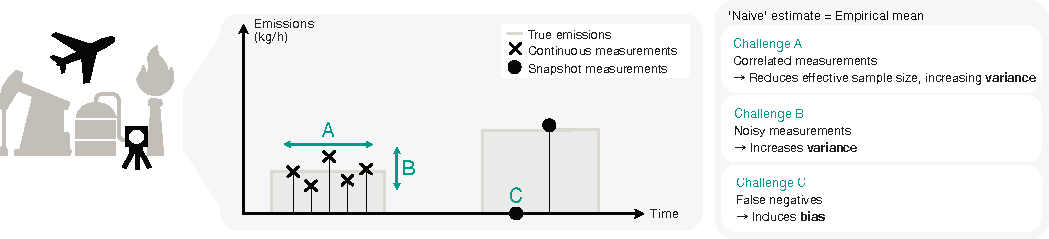
\includegraphics[width=\textwidth]{figures/figure0.pdf}
\caption{\edit{Conceptual overview of the estimation challenges. An intermittent source switches between active and inactive states over time. Continuous monitors (crosses) and snapshot measurements (circles) sample this process irregularly. Three challenges arise: \textbf{(A)}~multiple measurements may observe the same emission event, so positive dependence inflates the variance of the empirical mean and independent-sample assumptions overstate the effective sample size (details in SI, Section~\ref{SI-sec:corr_mean_SI}); \textbf{(B)}~detected emissions are measured with noise, increasing the variance of estimators built from them; \textbf{(C)}~small emissions fall below the detection threshold, producing false negatives that systematically shift the observed sample toward large values, biasing naive estimators of the time-averaged emission rate. Our framework addresses these challenges jointly.}}
\par\smallskip
{\small\textit{Alt text:} Schematic time series of an intermittent methane source alternating between active and inactive periods. Crosses mark continuous-monitor observations and circles mark snapshot observations. Three labelled callouts illustrate repeated sampling of the same emission event, measurement noise on detected emissions, and missed detections of small emissions below the detection threshold.}
\label{fig:challenges}
\end{figure}

\subsection{Statistical Model}
\label{sec:stat_model}

We model the data-generating process as a four-layer hierarchical process (Figure~\ref{fig:model_overview}). First, a latent ON/OFF state governs whether the source is emitting. Next, when the emission is active, the emission rate is drawn from a continuous distribution at event onset and persists at a constant rate until the event ends. We adopt this constant-rate specification for tractability, but it can also be interpreted flexibly: a source whose rate varies over time corresponds to a sequence of model events separated by brief OFF periods. Third, the observation process then filters this signal through sensor-dependent detection probability. And fourth, the size of the emission is estimated with possible quantification noise. A key estimation challenge is that detection probability depends on emission size, so non-detections are ambiguous: they may reflect true inactivity or a missed emission. Our framework addresses this by formally defining the likelihood of the observed sample, decomposing it into tractable components, and optimizing unknown parameters with an iterative strategy.

\begin{figure}[htbp]
\centering
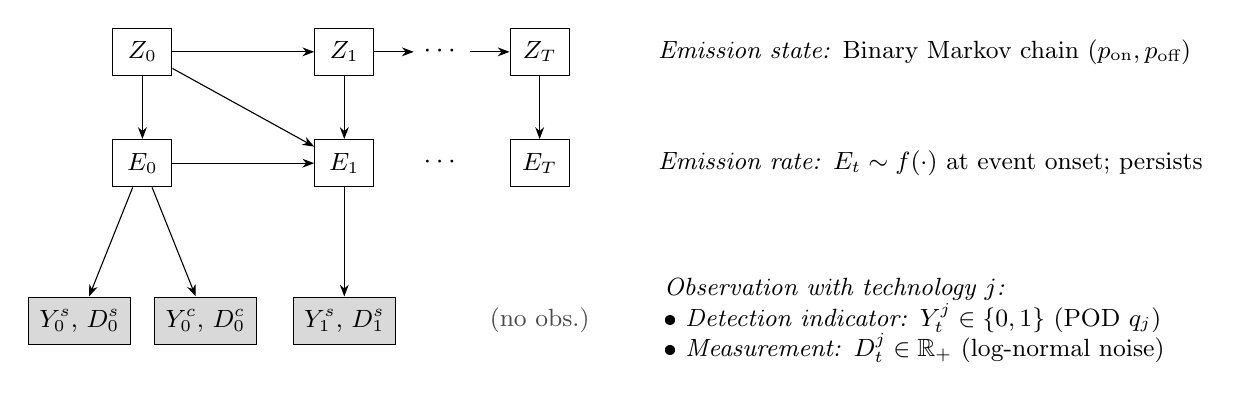
\begin{tikzpicture}[
    node distance=0.8cm and 1.8cm,
    box/.style={draw, minimum width=0.75cm, minimum height=0.6cm, font=\small},
    obs/.style={box, fill=gray!30},
    obswide/.style={draw, fill=gray!30, minimum width=1.3cm, minimum height=0.6cm, font=\small},
    arrow/.style={-{Stealth[length=1.5mm]}},
]
% Layer 1: Emission state
\node[box] (Z0) {$Z_0$};
\node[box, right=of Z0] (Z1) {$Z_1$};
\node[right=0.5cm of Z1] (Zdots) {$\cdots$};
\node[box, right=0.5cm of Zdots] (ZT) {$Z_T$};
\draw[arrow] (Z0) -- (Z1);
\draw[arrow] (Z1) -- (Zdots);
\draw[arrow] (Zdots) -- (ZT);

% Layer 2: Emission rate
\node[box, below=of Z0] (E0) {$E_0$};
\node[box, below=of Z1] (E1) {$E_1$};
\node (Edots) at ([yshift=-1.4cm] Zdots) {$\cdots$};  % explicitly aligned with E0/E1
\node[box, below=of ZT] (ET) {$E_T$};
\draw[arrow] (Z0) -- (E0);
\draw[arrow] (Z1) -- (E1);
\draw[arrow] (ZT) -- (ET);
\draw[arrow] (E0) -- (E1);
\draw[arrow] (Z0) -- (E1);

% Layer 3: Detection + measurement
\node[obswide] (O0s) at ([xshift=-0.8cm, yshift=-2.0cm] E0) {$Y_0^s,\, D_0^s$};
\node[obswide] (O0c) at ([xshift=+0.8cm, yshift=-2.0cm] E0) {$Y_0^c,\, D_0^c$};
\draw[arrow] (E0) -- (O0s);
\draw[arrow] (E0) -- (O0c);

\node[obswide] (O1s) at ([xshift=0cm, yshift=-2.0cm] E1) {$Y_1^s,\, D_1^s$};
\draw[arrow] (E1) -- (O1s);

\node[font=\small, text=gray!60!black] (noobs) at ([yshift=-2.0cm] ET) {(no obs.)};

% Right-side annotations — anchored to exact y of each layer
\node[right=1.0cm of ZT, font=\small, align=left] {%
    \textit{Emission state:} Binary Markov chain $(p_{\text{on}}, p_{\text{off}})$};
\node[right=1.0cm of ET, font=\small, align=left] {%
    \textit{Emission rate:} $E_t \sim f(\cdot)$ at event onset; persists};
\node[right=0.7cm of noobs, font=\small, align=left] {%
    \textit{Observation with technology $j$:}\\
    \textbullet~\textit{Detection indicator:} $Y_t^j\in\{0,1\}$ (POD $q_j$)\\
    \textbullet~\textit{Measurement:}
    $D_t^j\in\mathbb{R}_+$ (log-normal noise)};

\end{tikzpicture}
\caption{Graphical model for intermittent emissions with imperfect detection. Shaded nodes are observed; unshaded nodes are latent. The emission state $Z_t$ follows a two-state Markov chain. The emission rate $E_t$ is drawn at event onset and persists until the event ends. At each time step, the true rate may produce zero, one, or two pairs of detection/measurement outcomes depending on which technologies are deployed: $Y_t^j$ (detection indicator) and $D_t^j$ (measured value) for technology $j \in \{s, c\}$. Here $t = 0$ illustrates a dual-observation time step, $t = 1$ a single-technology observation, and $t = T$ an unobserved time step. When both technologies are present their detections are conditionally independent given $E_t$.}
\par\smallskip
{\small\textit{Alt text:} Directed graphical model in three rows. The top row is a chain of latent binary emission states from Z zero to Z T. The middle row holds emission rates E zero to E T, each depending on its own state, with E one also depending on E zero and Z zero. The bottom row holds shaded observed detection and measurement nodes: two technologies at time zero, one at time one, and none at time T.}
\label{fig:model_overview}
\end{figure}

\paragraph{Emission process.}
We model an emission source as switching between ON and OFF states over discrete time steps $t = 1, \ldots, T$. Let $Z_t \in \{0, 1\}$ denote the latent (unobserved) state, where $Z_t = 1$ indicates an active emission. The state sequence follows a two-state Markov chain with transition probabilities $p_{\text{on}} = p(Z_t = 1 \mid Z_{t-1} = 0)$ and $p_{\text{off}} = p(Z_t = 0 \mid Z_{t-1} = 1)$. The stationary probability of being ON is $\pi_{\text{on}} = p_{\text{on}} / (p_{\text{on}} + p_{\text{off}})$, and the mean emission duration is $\tau = 1/p_{\text{off}}$ time steps.


When $Z_t = 1$, the emission rate $E_t$ is drawn from an unknown distribution $f(\cdot)$ ($f(e)\doteq p(E_t=e|Z_t=1)$) at the start of each emission event and persists until the event ends. When $Z_t = 0$, $E_t = 0$. \edit{In our simulations we adopt a lognormal specification for $f$, which matches the right-skewed, heavy-tailed behavior observed empirically for oil-and-gas emissions \citep{Brandt2016, ZavalaAraiza2015}. The fitted rate law is an event-level IPW-weighted empirical distribution, so fitting does not require a lognormal family. The transition likelihood uses its full empirical support to preserve dependence within events. Other nonnegative generating distributions can be studied with the same algorithm, although recovery depends on detection coverage and the observed rate support. Some sites and basins are better described by heavier-tailed or mixture forms \citep{Sherwin2024Nature}, and we discuss the implications in Section~\ref{sec:discussion}.} Our target estimand is the time-averaged emission rate:
\begin{equation}
    \mu
    \doteq \mathbb{E}[E_t]
    = \mathbb{E}[\mathbb{E}[E_t\mid Z_t]]
    = \frac{p_\text{on}}{p_\text{on}+p_\text{off}}\cdot \mu_\text{emit},
    \label{eq:target}
\end{equation}
where $\mu_\text{emit}\doteq\mathbb{E}[E_t\mid Z_t=1]$.

\paragraph{Observation process.}
Each observation is characterized by three modular components: a detection probability curve, a noise model, and a sampling cadence. Different technologies differ in these three characteristics, and our framework treats these as modular inputs.

\new{We organize technologies into two regimes by the cadence at which they sample relative to emission duration. \emph{Snapshot} observations occur sparsely enough that each observation typically samples a different emission event; \emph{continuous} observations occur densely enough that multiple observations typically fall within a single event. The distinction is a property of the cadence, not of the platform: an aerial survey flown in a lawn-mower pattern can be effectively continuous for a revisited site, while a continuous monitor with long wind-direction gaps might be effectively acting as a snapshot technology, especially for short-duration events. The framework treats both regimes through the same likelihood, so the platform label does not affect the inference.}

\new{We adopt simple stochastic specifications for both sampling regimes; the framework treats the resulting sequence of observation timestamps as inputs and is agnostic to the mechanism that generated them.} At each time step $t$, a snapshot observation is modelled as occurring independently with probability $p_{\text{snap}}$ (representing discrete aerial or satellite visits). Continuous monitors are modeled as a renewal process: at each unmonitored time step, a Bernoulli draw with probability $p_{\text{cont}}$ triggers deployment of a monitor that then runs for $T_{\text{cont}}$ contiguous time steps; during an active window no new deployment draw is made, and snapshots can still occur. \new{This Bernoulli-onset, fixed-duration structure is a coarse abstraction of the physical process governing sensor visibility. Continuous monitors detect the plume only when wind direction aligns the source with the sensor; this alignment appears and disappears stochastically as winds shift, and tends to persist for a characteristic duration once established. The two parameters $p_{\text{cont}}$ and $T_{\text{cont}}$ summarize these two aspects; richer specifications (e.g.\ drawing $T_{\text{cont}}$ from a distribution) are straightforward extensions that do not modify the estimator. Real-world deployment patterns are not strictly Bernoulli, but the framework only uses the resulting sequence of observation timestamps; pre-set schedules, periodic surveys, or other deterministic deployment patterns yield the same inference as long as the timing is independent of the emission state. We sweep both parameters in SI, Sections~\ref{SI-sec:sweep_pcont_SI} and~\ref{SI-sec:sweep_Tcont_SI}.} At each time step we may have no observation, a single technology, or both. When both technologies observe simultaneously, their detections are conditionally independent given the latent emission rate, but not generally after averaging over unknown event size.
\textit{Detection.} At each observed time, the sensor either detects an emission ($Y_t = 1$) or not ($Y_t = 0$). When $Z_t=1$ (active emission), the detection probability depends on the emission size through a probability-of-detection (POD) curve $q(e)$, assumed known from controlled release experiments. We model POD as a logistic function:
\begin{equation}
    q_j(e)
    \doteq p(Y^j_t=1\mid Z_t=1,E_t=e)
    = \frac{1}{1+(\theta_j/e)^{k_j}},
    \label{eq:pod}
\end{equation}
where $\theta_j \in\mathbb{R}_+$ is the 50\% detection threshold and $k_j\in\mathbb{R}_+$ controls steepness. For simplicity, we assume here that the sensing technologies are not subject to false positives, i.e.\ $Y_t=0$ when $Z_t=0$. This assumption could be relaxed in future models.

\textit{Measurement noise.} When an emission is detected, the measured value $D_t$ differs from the true emission rate $E_t$ due to atmospheric variability, algorithm limitations, and instrument bias and noise. For simplicity here, we model this as multiplicative log-normal noise:
\begin{equation}
    D^j_t = E_t \cdot \exp(\varepsilon_t), \quad \varepsilon_t \sim \mathcal{N}(-\sigma_j^2/2, \sigma_j^2),
    \label{eq:noise}
\end{equation}
where $\sigma_j$ characterizes measurement uncertainty. This formulation ensures measured values remain positive and yields an unbiased measurement process. \new{Controlled-release tests of aerial and satellite platforms typically show approximately symmetric error distributions rather than strictly multiplicative lognormal noise \citep{Sherwin2023, ElAbbadi2024}; at the small log-scale standard deviations relevant for these technologies ($\sigma \approx 0.05$--$0.1$), the lognormal and additive normal models are numerically very close, and the algorithmic structure of our framework does not depend on which is used. The lognormal form is more directly motivated for continuous monitors, where relative errors of order 20\% are observed across a wide range of emission sizes \citep{Daniels2024}. Fenceline continuous monitors are an exception: their error distributions are typically left-censored, with rates below an instrument-specific floor reported as zero, and the framework accommodates this through substitution of a censored noise model for equation~\eqref{eq:noise}. The sensitivity of the estimator to misspecification of the noise parameters is quantified in SI, Section~\ref{SI-sec:misspec_SI}.}

\textit{Sampling schedule.} Continuous monitors do not automatically detect all emission events: emissions can be transported between or above sensors as winds change, and even imaging-based continuous monitors can exhibit blind spots due to sensor placement interactions with plume transport. Snapshot measurements — from satellites, aircraft, or mobile surveys — have higher detection thresholds but can cover many facilities, and differ in spatial specificity in ways we do not address here.



\paragraph{The estimation challenge.}
With imperfect detection, a non-detection is ambiguous: it could mean the source was OFF, or that an emission was too small to be detected. To account for this ambiguity it is useful to introduce $\kappa_j$ as the marginal probability for an active source to be detected by technology $j$:
\begin{equation}
    \kappa_j
    \doteq p(Y_{t}^j=1\mid Z_t=1)
    = \int p(Y_{t}^j=1,E_t=e\mid Z_t=1)\,\mathrm{d}e
    = \int q_j(e)\,f(e)\,\mathrm{d}e.
    \label{eq:kappa}
\end{equation}
Estimating the components $\mu_{\text{emit}}$, $p_{\text{on}}$, and $p_{\text{off}}$ separately requires information about the emission-size distribution $f$, because detection probabilities depend on the full distribution rather than its mean alone. We estimate this distribution empirically from linked emission events using inverse-probability weighting. This avoids imposing a parametric family during fitting, but recovery depends on the assumed POD curves, measurement model, and the ability of detected events to represent the underlying size distribution. Emissions with zero detection probability cannot be recovered from these records alone.

At time steps where multiple technologies observe simultaneously, their detections are conditionally independent given the true emission size $E_t$. After marginalizing over $E_t$, detection outcomes are correlated: large emissions are easy for both sensors to detect, while small emissions are hard for both. The same shared size also induces dependence across observations of an ongoing event. For example, two snapshot detections within the same event involve $\mathbb{E}[q_s(E)^2]$, rather than $\mathbb{E}[q_s(E)]^2$. The transition likelihood therefore retains the estimated distribution of persistent event sizes, rather than replacing it by marginal detection probabilities alone (SI, Section~\ref{SI-sec:forward}).


\subsection{Estimation}
\label{sec:estimation}

\paragraph{Maximum likelihood estimation.}
Maximum likelihood estimation (MLE) seeks the parameter values that make the observed data most probable. Given a statistical model with parameters $\boldsymbol{\theta}$ and a set of observation $\Omega$, the maximum-likelihood estimate is defined as $\hat{\boldsymbol{\theta}} = \arg\max_{\boldsymbol{\theta}} \mathcal{L}(\boldsymbol{\theta})$, where $\mathcal{L}$ is the likelihood function, i.e. the probability of observing $\Omega$ under $\boldsymbol{\theta}$: $\mathcal{L}(\boldsymbol{\theta})=p(\Omega|\boldsymbol{\theta})$. Under standard regularity conditions, the MLE is asymptotically unbiased and efficient: it attains the inverse-Fisher-information variance among regular estimators \citep{vanderVaart1998}. \new{Asymptotic unbiasedness refers to the vanishing of bias as the sample size grows; at finite sample sizes, the MLE typically exhibits a bias of order $O(1/N)$ \citep[Ch.~5]{vanderVaart1998}, but this standard theory does not establish unbiasedness or efficiency of the iterative plug-in procedure used here. Its finite-sample performance is evaluated by simulation.}

In our setting, computing the full likelihood requires marginalizing over the complete latent state path $\mathbf Z=(Z_1,\ldots,Z_T)$ and rate path $\mathbf E=(E_1,\ldots,E_T)$, conditional on the sampling masks:
\begin{equation}
    \mathcal L(p_{\text{on}},p_{\text{off}},f)
    =\sum_{\mathbf Z\in\{0,1\}^T}
      P(\mathbf Z\mid p_{\text{on}},p_{\text{off}})
      \int P(\mathbf Y,\mathbf D\mid\mathbf Z,\mathbf E)
      \,\mathrm dF_f(\mathbf E\mid\mathbf Z).
    \label{eq:full_likelihood}
\end{equation}
Here $F_f(\mathbf E\mid\mathbf Z)$ is the joint rate-path distribution induced by the event-size law $f$: rates are zero while OFF and shared throughout each ON event. Using a distribution measure accommodates these point masses and equality constraints without treating rates at successive times as independent continuous draws.
Evaluating this expression requires summing over event histories and integrating over their emission sizes. Although the integral has no general closed form, the likelihood can be approximated numerically by including emission size in the hidden state and using a forward recursion \citep{LangrockKing2013}. We instead estimate $f$ by plume linking and event-level IPW, then maximize the detection likelihood conditional on that estimate. Repeating these steps gives the three-step procedure below. It does not jointly maximize equation~\eqref{eq:full_likelihood} and is not an exact expectation--maximization algorithm. Here, ``MLE'' refers to the estimator with these conditional maximum-likelihood transition updates.

\paragraph{Step 1: Plume identification.}
Detections from all technologies are merged into a single time-sorted list. Detections at the same time step from different technologies are always assigned to the same plume (they observe the same hidden state). When both technologies detect simultaneously, their measurements are combined via inverse-variance weighting in log-space (since the noise model is multiplicative), giving more weight to the lower-noise technology.

The combined simultaneous measurements and their effective noise are used for the approximate Bayesian linking step: for detections at different time steps, we assign them to plumes using a model that combines temporal proximity and measurement similarity. Detections are merged when the working posterior probability of belonging to the same plume exceeds a decision threshold $\delta = 0.5$. Sensitivity to $\delta$ is assessed in SI, Section~\ref{SI-sec:threshold}. The derivation of the Bayes factor and implementation details are given in SI, Section~\ref{SI-sec:bayes_factor}.

After event linking, when a plume comprises $n > 1$ measurements (either from simultaneous multi-technology detections or from linked detections across time steps, see next paragraph) the inverse-variance weighted mean in log-space is exponentiated to obtain the plume size estimate. Conditional on correct plume assignments, exponentiating an average log measurement produces a downward shift by Jensen's inequality ($\exp(\mathbb{E}[\log X]) \leq \mathbb{E}[X]$) \citep{CoverThomas2006}. Under the lognormal noise model, the bias has a closed-form correction: we multiply by $\exp\bigl((n-1)/(2W)\bigr)$, where $W = \sum_{j=1}^{n} \sigma_j^{-2}$ is the total precision of the $n$ measurements.

\paragraph{Step 2: Bias-corrected emission-size distribution.}
The identified plumes provide a sample of emission sizes biased toward large values, because small emissions are less likely to be detected. Unlike the POD-weighted baseline, which operates per-observation and avoids the event-duration issue entirely (at the cost of higher variance from redundant observations; see SI, Section~\ref{SI-sec:alternatives} for further discussion), our method groups detections into events and estimates $\mathbb{E}[E \mid Z=1]$ from this event-level sample. This grouping is what enables variance reduction, but it introduces a new bias concern: the probability of detecting an event at least once depends on how long it persists, because longer events have more detection opportunities. A simple per-step correction $1/q(e)$ would overcorrect for persistent events and undercorrect for brief ones.

We address this using inverse-probability weighting (IPW) at the event level, \new{an approach analogous to the per-detection IPW correction used by \citet{Sherwin2024Nature} for aerial data}. Each plume $m$ with estimated size $\hat{e}_m$ receives weight $w_m = 1/P_{\text{det}}(\hat{e}_m)$, where $P_{\text{det}}(e)$ is the probability that an emission event of size~$e$ is detected at least once during its lifetime. Small emissions that are hard to detect receive large weights, compensating for similar events that were missed entirely. The corrected mean emission rate is
\begin{equation}
    \hat{\mu}_{\text{emit}}
    = \frac{\sum_m w_m \,\hat{e}_m}{\sum_m w_m}.
    \label{eq:ipw}
\end{equation}
Intuitively, each detected event ``represents'' itself plus the similar-sized events that were missed: if an event of size $e$ is detected with probability $P_{\text{det}}(e) = 0.5$, on average one equally-sized event went undetected, and the weight $w = 2$ accounts for it. The computation of $P_{\text{det}}(e)$ is detailed in SI, Section~\ref{SI-sec:event_ipw}.

\paragraph{Step 3: Transition probability estimation.}
Normalize the event-level IPW weights to $\tilde w_m=w_m/\sum_\ell w_\ell$, giving the empirical distribution $\hat f=\sum_{m=1}^{M}\tilde w_m\,\delta_{\hat e_m}$. Conditional on this distribution, we maximize the likelihood of the observed detection sequence over $(p_{\text{on}},p_{\text{off}})$. The hidden state comprises OFF and $M$ ON states, one for each estimated plume size. A source that remains ON retains its size; following an OFF-to-ON transition, a new size is drawn according to $\tilde w_m$. Detection probabilities are evaluated at each support point, preserving both simultaneous sensor dependence and temporal dependence within events.

The forward recursion costs $O(NM)$ per likelihood evaluation for $N$ observation times and $M$ support points. Integer gaps are handled by exact multi-step transitions of this finite-state model, including the possibility that an event ends and a new one begins between observations (SI, Sections~\ref{SI-sec:forward} and~\ref{SI-sec:multistep}). We use continuous optimization in log probabilities on the fixed domain $[10^{-5},1-10^{-6}]^2$, with a fixed coarse search for an additional starting point in the first iteration. The bounds and starting values are fixed independently of the generating parameters, and no multiplicative adjustment is applied to the likelihood. The recursion is exact conditional on $\hat f$, which is estimated from linked, noisy measurements. Numerical sensitivity is reported in SI, Section~\ref{SI-sec:robustness_grid}.

\paragraph{Iteration and final estimate.}
Steps~1--3 are repeated, with the updated $\hat p_{\text{off}}$ feeding back into plume linking and the event-detection weights. Iteration stops when both transition probabilities change by less than $10^{-5}$ and the estimated overall mean changes by less than $10^{-4}$~kg/h, with a maximum of 30 iterations. The outer loop is not guaranteed to increase a joint likelihood at every iteration. Estimates reaching the iteration limit or a search boundary are retained in the simulation summaries, and their frequencies are reported in the SI. For observed campaigns with no detections we define $\hat\mu=0$ and leave the component parameters unidentified. The final estimate is
\begin{equation}
    \hat{\mu}
    = \frac{\hat{p}_{\text{on}}}
           {\hat{p}_{\text{on}} + \hat{p}_{\text{off}}}
      \cdot \hat{\mu}_{\text{emit}}.
    \label{eq:final}
\end{equation}
Uncertainty is quantified via nested replication (typically, 500 inner replicates with 25 outer replicates).

\begin{figure}[htbp]
\centering
\fbox{\parbox{0.92\textwidth}{%
\textbf{Algorithm: Self-Consistent MLE for Intermittent Emissions}
\vspace{0.3em}

\textbf{Input:} Observation sequence $\{(t_i, j_i, Y_i, D_i)\}$, POD curves $q_j(\cdot)$, noise parameters $\sigma_j$

\textbf{Initialize:} $(\hat p_{\text{on}}^{(0)},\hat p_{\text{off}}^{(0)})=(0.025,0.10)$
\vspace{0.3em}

\textbf{Repeat} until transition changes are below $10^{-5}$ and the mean change is below $10^{-4}$~kg/h, or 30 iterations are reached:
\begin{enumerate}
    \item \textit{Plume identification.} Link detections into events via Bayesian posterior using temporal prior from $\hat{p}_{\text{off}}^{(k-1)}$; combine multi-technology measurements via inverse-variance weighting; apply Jensen bias correction.
    \item \textit{Emission distribution.} Compute $P_{\text{det}}(e)$ via backward recursion; estimate $\hat\mu_{\text{emit}}$ and the weighted empirical size distribution $\hat f$ via event-level IPW.
    \item \textit{Transition probabilities.} Maximize the persistent-size detection likelihood conditional on $\hat f$ over fixed bounds, using the forward recursion.
\end{enumerate}
\vspace{0.3em}

\textbf{Output:} $\hat{\mu} = \hat{\pi}_{\text{on}} \cdot \hat{\mu}_{\text{emit}}$
}}
\end{figure}

\newpage

\section{Results}
\label{sec:results}


\subsection{Experimental Setup}

\subsubsection{Simulation Framework}

We evaluate our method using Monte Carlo simulations, where each simulation generates a complete emission time series, simulates the observation process for multiple monitoring technologies, and applies each estimation method to the resulting data to recover (infer) the simulation parameters.

The simulation proceeds as follows. First, we generate a latent emission state sequence $\{Z_t\}_{t=1}^T$ from a two-state Markov chain with parameters $(p_{\text{on}}, p_{\text{off}})$. For each time step where $Z_t = 1$ and $Z_{t-1}=0$ (new emission starts), we sample an emission rate $E_t$ from a lognormal distribution. Second, we simulate the observation process: at each time step $t$, a snapshot observation occurs with probability $p_{\text{snap}}$ (independent Bernoulli trial). Continuous monitoring follows a renewal process: at each unmonitored step, a Bernoulli trial with probability $p_{\text{cont}}$ triggers deployment of a monitor that then runs for $T_{\text{cont}}$ contiguous steps. Both technologies can be active simultaneously during a continuous window. Third, for each observation, we simulate detection according to the technology-specific POD curve and, if detected, add multiplicative measurement noise. This yields a dataset of detection times, measured emission sizes, and technology identifiers---the same information available in real emissions monitoring programs.

\subsubsection{Baseline Scenario Parameters}

\edit{Table~\ref{tab:baseline_params} summarizes the parameters for our baseline scenario. Time steps are one hour, and $p_{\text{snap}} = 0.125$ corresponds in expectation to three snapshot observations per day. This cadence is at the upper end of what current tasked satellite constellations can achieve for high-priority facilities (e.g., GHGSat combined with Carbon Mapper), though above the cadence of any single platform in routine operation. We explore sparser cadences, down to monthly surveys, in the $p_{\text{snap}}$ sweep of Section~\ref{sec:sweeps_main} and the very-sparse example in SI, Section~\ref{SI-sec:sparse_SI}.}

\begin{table}[h]
\centering
\caption{Baseline simulation parameters. \new{Time steps are one hour throughout.}}
\label{tab:baseline_params}
\begin{tabular}{llrl}
\toprule
\multicolumn{4}{l}{\textit{Emission process}} \\
\midrule
$T$ & Time horizon & 1000 & hours \\
$\mu_{\text{emit}}$ & Mean emission rate (when ON) & 50 & kg/h \\
$\tau$ & Mean ON duration & 20 & hours \\
$\pi_{\text{on}}$ & Stationary ON probability & 20\% & \\
\midrule
\multicolumn{4}{l}{\textit{Observation process}} \\
\midrule
$p_{\text{snap}}$ & Snapshot observation prob.\ per time step & \edit{12.5\%} & \\
$p_{\text{cont}}$ & Per-step prob.\ of starting continuous window & 1\% & \\
$T_{\text{cont}}$ & Duration of continuous monitor & 50 & time steps \\
$\theta_{\text{snap}}$ & Snapshot 50\% POD threshold & 50 & kg/h \\
$\theta_{\text{cont}}$ & Continuous 50\% POD threshold & 2.4 & kg/h \\
$\sigma_{\text{snap}}$ & Snapshot meas.\ noise (log-scale) & 0.05 & \\
$\sigma_{\text{cont}}$ & Continuous meas.\ noise (log-scale) & 0.2 & \\
\botrule
\end{tabular}
\end{table}


\edit{Detection thresholds in the table span current technology ranges: 50--200~kg/h for aircraft and satellites, and below 10~kg/h for ground-based CMS \citep{chen2024comparing, Conrad2023, ElAbbadi2024, Sherwin2023}. Measurement noise parameters ($\sigma_{\text{snap}} = 0.05$, $\sigma_{\text{cont}} = 0.2$) cover the range observed in controlled-release validation studies \citep{Sherwin2021, Sherwin2023}. Emission durations of hours to days are consistent with field observations of equipment malfunctions \citep{Cusworth2021, Cusworth2026NatComms, Daniels2024}. We note that the ``continuous'' and ``snapshot'' categories can represent many concrete pairings — ground-based continuous monitoring systems (CMS) versus aircraft, frequent satellite revisits versus infrequent overflights, or two satellite constellations with different tasking frequencies — so long as their sampling cadences differ by an order of magnitude or more. Example realizations, POD curves, and the emission size distribution are provided in SI, Section~\ref{SI-sec:sim_figures}.}

\subsubsection{Baseline Methods}

We compare our method against two baselines that represent common approaches in the literature.

\paragraph{Naive estimator.}
The simplest approach sums detected emissions and divides by total observation time:
\begin{equation}
    \hat{\mu}_{\text{naive}} = \frac{1}{N_{\text{obs}}} \sum_{i: Y_i = 1} D_i,
\end{equation}
where the sum runs over observations with detections and $D_i$ is the measured emission size. This estimator underestimates total emissions because it misses active emissions that fall below the detection threshold; these contribute zero to the sum rather than their true (positive) value. Within the sensing system's full detection range, however, the naive average is an unbiased estimator of mean emissions, as established by \citet{Chen2022EST} and \citet{Sherwin2024Nature}.


\paragraph{POD-weighted estimator.}
A natural improvement applies inverse-probability weighting to correct for missed detections, as done for aerial data in \citet{Sherwin2024Nature}:
\begin{equation}
    \hat{\mu}_{\text{POD}} = \frac{1}{N_{\text{obs}}} \sum_{i: Y_i = 1} \frac{D_i}{q(D_i)},
\end{equation}
where $q(D_i)$ is the probability of detecting an emission of measured size $D_i$. Each detected emission is upweighted by the inverse of its detection probability, compensating for similar-sized emissions that were missed. Intuitively, at any observed time step, if the source emits at rate $e$ and is detected with probability $q(e)$, the expected contribution $e \cdot q(e) / q(e) = e$ recovers the true rate regardless of whether the source is ON or OFF when the rate is measured without error. Evaluating $q$ at a noisy measurement is a further plug-in approximation, so this identity alone does not establish exact unbiasedness of the implemented POD-weighted estimator. Crucially, this per-observation argument requires no knowledge of event duration, because observations are never grouped into events. The price is that repeated observations of the same persistent emission contribute correlated, redundant samples, inflating variance. \new{This is precisely the mechanism motivated in Section~\ref{sec:introduction} and formalized in SI, Section~\ref{SI-sec:corr_mean_SI}: an unweighted mean need not make efficient use of correlated observations, and the excess variance grows with the degree of correlation between observations of the same persistent event. \citet{Sherwin2024Nature} similarly use this per-observation IPW correction in the partial-detection range, combined with a naive average for emissions in the full detection range and a spliced simulated tail below the detection limit; our framework combines event-level IPW with conditional transition-likelihood fitting over the modeled detection range.}

\paragraph{MLE-ungrouped estimator.}
To assess the combined contribution of the iterative event-level procedure (Steps~1--3 above), we introduce an intermediate method that uses per-detection IPW like the POD-weighted estimator but then feeds the resulting weighted empirical size distribution into the persistent-size forward algorithm to estimate $(p_{\text{on}}, p_{\text{off}})$.

MLE-ungrouped proceeds in two steps. First, it estimates $\hat{\mu}_{\text{emit}}$ and the weighted empirical size distribution from individual detections. When both technologies detect simultaneously, their measurements are combined via inverse-variance weighting in log-space, and the combined detection probability $q_{\text{comb}} = 1 - (1-q_s)(1-q_c)$ is used for IPW:
\begin{equation}
    \hat{\mu}_{\text{emit}}^{\text{simple}} = \frac{\sum_{i} D_i / q_{\text{det},i}}{\sum_{i} 1/q_{\text{det},i}},
    \qquad
    \hat f_{\text{simple}} = \frac{\sum_i q_{\text{det},i}^{-1}\delta_{D_i}}{\sum_i q_{\text{det},i}^{-1}}.
    \label{eq:mle_simple}
\end{equation}
Second, it estimates $(p_{\text{on}}, p_{\text{off}})$ by maximizing the persistent-size detection likelihood conditional on $\hat f_{\text{simple}}$, using the same fixed bounds as in Step~3, and combines:
$\hat{\mu}_{\text{simple}} = \hat{\pi}_{\text{on}} \cdot \hat{\mu}_{\text{emit}}^{\text{simple}}$.

This method is non-iterative (one-shot) and avoids the plume identification step entirely. Differences between the grouped estimator and MLE-ungrouped therefore reflect the event-level grouping, measurement averaging within plumes, and the duration-aware IPW correction.

Table~\ref{tab:methods_comparison} summarizes the key differences between the methods considered.

\begin{table}[h]
\centering
\caption{Comparison of estimation methods. Columns indicate whether each
method adjusts for size-dependent detection bias, accounts for temporal
correlation among observations of the same emission event, and reduces
measurement noise by averaging multiple observations within identified events.\new{ Blank cells indicate the method does not provide the capability; \ding{51} indicates it does.}}
\label{tab:methods_comparison}
\small
\begin{tabular}{lccc}
\toprule
Method & Corrects & Accounts for & Reduces noise via \\
       & detection bias & emission correlation & event-level averaging \\
\midrule
Naive          &           &           &           \\
POD-weighted   & \ding{51} &           &           \\
MLE-ungrouped (ours)  & \ding{51} & \ding{51} &           \\
MLE (ours)     & \ding{51} & \ding{51} & \ding{51} \\
\botrule
\end{tabular}
\end{table}

\subsubsection{Evaluation Protocol}

For the baseline configuration, we use a nested replication design: $B = 25$ outer batches of $N = 500$ independent simulations each, yielding $N_{\text{total}} = 12{,}500$ simulations. Within each outer batch, we compute the mean and variance of each estimator. Bias is then estimated as the average (across outer batches) of the inner-batch means minus the true value, and its standard error is estimated from the outer-batch variability. This design provides robust uncertainty quantification for both bias and variance estimates.

For parameter sweeps, we vary a single parameter while holding all others at baseline, using the same nested replication design ($25 \times 500$).


\subsection{Performance under Baseline Conditions}
\label{sec:baseline_performance}

\edit{Figure~\ref{fig:baseline} summarizes performance across 12{,}500 simulations under baseline conditions ($p_{\text{snap}} = 0.125$, true time-averaged emission rate $\mu = 0.20 \times 50 = 10.0$~kg/h).}

\begin{figure}[htbp]
\centering
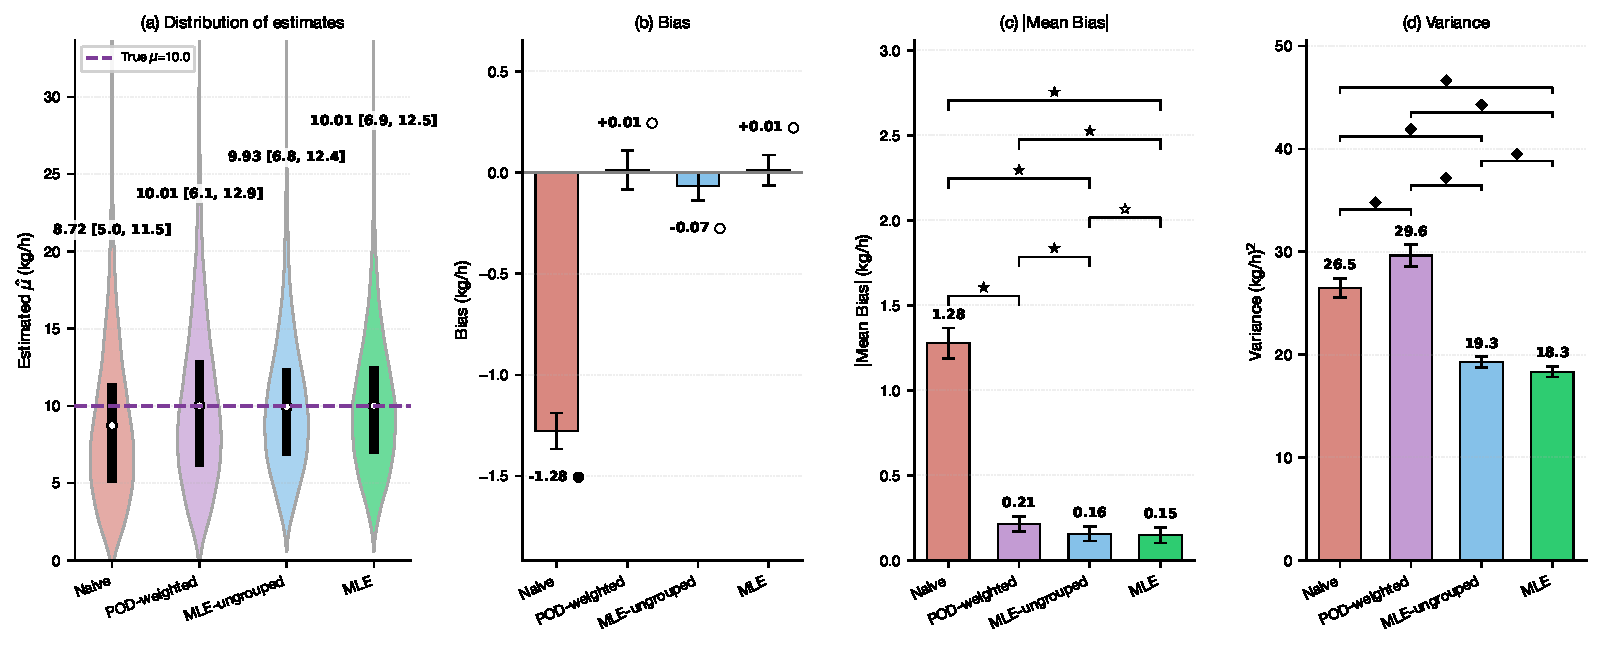
\includegraphics[width=\textwidth]{figures/figure_baseline_violin_v2_wide.pdf}
\caption{Bias--variance comparison of estimation methods ($N = 12{,}500$ simulations, 25 outer batches of 500). \new{The central result is panel~(d): the MLE reduces the variance of $\hat{\mu}$ by \edit{34}\% relative to the probability-of-detection-weighted estimator (\edit{19.6} vs.\ \edit{29.6}~(kg/h)$^2$) with estimated bias $+0.077$~kg/h on a true mean of $10$~kg/h.}
\textbf{(a)}~Violin plots of $\hat{\mu}$; white dots mark the mean, thick bars the interquartile range (IQR), and bold annotations show mean~[IQR]. The dashed line indicates the true value $\mu = 10.0$~kg/h.
\textbf{(b)}~\edit{Signed mean bias (kg/h) for each method, averaged across outer batches.} Filled circles~($\bullet$) indicate the null hypothesis of unbiasedness is rejected at $p < 0.05$ (one-sample $t$-test on 25 batch means); open circles~($\circ$) indicate it cannot be rejected.
\textbf{(c)}~\edit{Absolute value of the signed mean bias, $|\bar{b}|$ (kg/h), averaged over 25 outer batches.} Brackets with filled stars~($\bigstar$) denote pairs whose absolute biases differ significantly ($p < 0.05$, paired $t$-test); open stars~($\star$) indicate no significant difference.
\textbf{(d)}~Variance of $\hat{\mu}$, averaged over 25 outer batches. Brackets with filled diamonds~($\blacklozenge$) denote pairs whose variances differ significantly ($p < 0.05$, paired $t$-test); open diamonds~($\lozenge$) indicate no significant difference. \new{The MLE--POD-weighted difference is significant at $p < 0.05$; the intermediate MLE-ungrouped variance (20.6) provides a comparator for the combined effects of event linking, within-event averaging, event-level IPW, and iteration. This comparison does not isolate linking alone.}
Error bars in panels (b)--(d) are 95\% Student-$t$ Monte Carlo confidence intervals from 25 outer batches (24 degrees of freedom). \new{Panel (b) averages signed batch biases, $25^{-1}\sum_k\bar b_k$, whereas panel (c) averages their magnitudes, $25^{-1}\sum_k|\bar b_k|$. These are different statistics: the latter includes Monte Carlo variation in finite batch means and is not the absolute value of the overall bias.}
Full test statistics and exact $p$-values are reported in SI, Section~\ref{SI-sec:pairwise_tests}, Tables~\ref{SI-tab:unbiasedness} and~\ref{SI-tab:pairwise_tests}.}
% Full test statistics and exact $p$-values are reported in SI, Section~\ref{SI-sec:pairwise_tests}, Tables~\ref{SI-tab:unbiasedness} and~\ref{SI-tab:pairwise_tests}.}
\par\smallskip
{\small\textit{Alt text:} Four-panel figure comparing the naive, probability-of-detection-weighted, MLE-ungrouped and MLE estimators of the time-averaged emission rate across 12,500 simulations. Panel a shows violin plots of the estimates around the true value of 10 kg/h. Panels b and c show signed mean bias and mean absolute batch bias; only the naive estimator is clearly biased, underestimating by about 1.3 kg/h. Panel d shows estimator variance, lowest for the MLE at 19.6 squared kg/h compared with 29.6 for the probability-of-detection-weighted estimator.}
\label{fig:baseline}
\end{figure}



\edit{The naive estimator underestimates the mean by $1.28$~kg/h. The POD-weighted, MLE-ungrouped, and MLE mean estimates are $10.01$, $9.98$, and $10.08$~kg/h, respectively, against the true value $10.0$~kg/h. The MLE has an estimated bias of $+0.077$~kg/h. The estimated squared bias is about $0.006$~(kg/h)$^2$, small relative to its variance of $19.6$~(kg/h)$^2$. This comparison describes performance in the baseline simulations. The average within-batch variances are $29.6$, $20.6$, and $19.6$~(kg/h)$^2$, corresponding to a $33.9\%$ reduction for MLE relative to POD weighting ($p<0.001$). The MLE variance is also $5.1\%$ lower than that of MLE-ungrouped ($p<0.001$). Both likelihood-based estimators use the persistent-size transition update; their difference reflects the combined effects of event linking, within-event measurement combination, event-level IPW, and iteration. It does not isolate linking alone. All $12{,}500$ mean estimates are included, including two zero-detection campaigns assigned zero; component parameters are unavailable for those two records. Fifty-seven campaigns with detections reach the outer iteration limit, two have a final optimizer flag, and two reach a transition bound; these finite estimates are retained.}

\new{The sign and functional form of this variance reduction across monitoring regimes are examined in Section~\ref{sec:sweeps_main}; robustness to misspecification of sensor parameters is characterized in SI, Section~\ref{SI-sec:misspec_SI}.}

\subsubsection{Recovery of Underlying Parameters}

\begin{figure}[htbp]
\centering
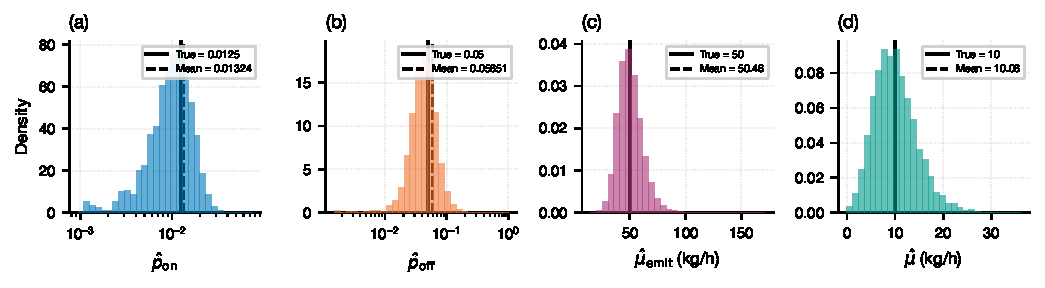
\includegraphics[width=\textwidth]{figures/figure1_histograms.pdf}
\caption{\new{\textbf{(a--d)}~}Distributions of MLE parameter estimates across $N = 12{,}500$ simulations ($25 \times 500$). From left to right: \new{(a)~}ON transition probability~$\hat{p}_{\text{on}}$, \new{(b)~}OFF transition probability~$\hat{p}_{\text{off}}$, \new{(c)~}conditional mean emission rate~$\hat{\mu}_{\text{emit}}$, and \new{(d)~}time-averaged emission rate~$\hat{\mu}$. Solid vertical lines mark the true values; dashed lines mark the sample means. Transition-probability axes are logarithmic to show the full range, including rare boundary estimates. The conditional mean and time-averaged rate are close to their true values, while the transition estimates exhibit positive shifts. Panels (a--c) include the $12{,}498$ campaigns with component estimates; panel (d) includes all $12{,}500$ mean estimates. The campaign-length sweep (SI, Section~\ref{SI-sec:sweep_T}) examines these shifts empirically; standard MLE asymptotics do not establish the behaviour of this plug-in estimator.
}
\par\smallskip
{\small\textit{Alt text:} Four histograms of maximum likelihood estimates across 12,500 simulations, for the ON transition probability, the OFF transition probability, the conditional mean emission rate and the time-averaged emission rate. Solid lines mark true values and dashed lines mark sample means. The conditional mean and overall mean are close to their true values; the transition probabilities show upward shifts, especially the OFF probability.}
\label{fig:param_histograms}
\end{figure}

Beyond the aggregate emission rate, our method estimates the underlying process parameters (Figure~\ref{fig:param_histograms}). Mean estimates of $p_{\text{on}}$ and $p_{\text{off}}$ are $0.01324$ and $0.05851$, against true values $0.0125$ and $0.05$. The conditional mean emission estimate is $50.46$~kg/h, against $50.0$~kg/h. The OFF transition probability is overestimated in the baseline simulations. Campaign length, event assignments, noisy size estimates, and the empirical size distribution can each contribute to this error. The campaign-length sweep in SI, Section~\ref{SI-sec:sweep_T}, examines how parameter recovery changes with the amount of data; it does not isolate these contributions.

The campaign-length sweep in SI, Section~\ref{SI-sec:sweep_T} and Figure~\ref{SI-fig:composite_T}, reports relative bias and coefficient of variation for each parameter. Longer campaigns can improve recovery, but finite simulated lengths do not establish consistency of the plug-in procedure.

%-----------------------------------------------------------------------------
\subsection{Sensitivity to Model Parameters}
\label{sec:sweeps_main}
%-----------------------------------------------------------------------------

\edit{We examine how the relative performance of our method varies across the parameter space by conducting systematic sweeps over three key variables: snapshot cadence, emission persistence, and snapshot detection threshold. In each sweep, a single parameter is varied while all others are held at baseline values. Sweeps over continuous-monitoring parameters ($p_{\text{cont}}$ and $T_{\text{cont}}$) are reported in the SI (Section~\ref{SI-sec:sweep_cont_SI}), where they complement the main-text analysis by characterizing how continuous-sensor coverage interacts with variance reduction.}

\begin{figure}[htbp]
\centering
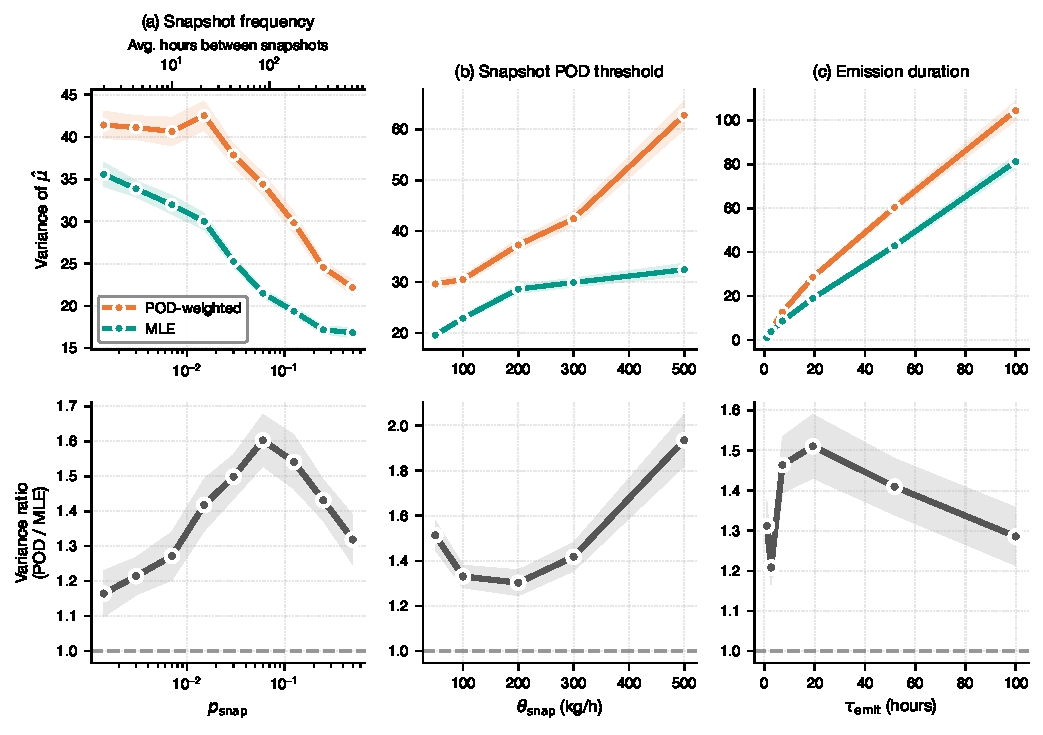
\includegraphics[width=\textwidth]{figures/figure4_composite.pdf}
\caption{Sensitivity of estimation variance to key parameters (shaded bands show normal-approximation 95\% Monte Carlo bands over $25$ outer batches; ratio bands use delta-method propagation of the marginal variance standard errors). Each column varies one parameter while holding all others at baseline values. Top row: variance of the MLE and POD-weighted estimators. Bottom row: variance ratio (POD-weighted / MLE); values above the dashed line indicate lower MLE variance. \edit{\textbf{(a)}~Snapshot observation probability $p_{\text{snap}}$ (top axis also shown in units of average time between snapshot observations). \textbf{(b)}~Snapshot 50\% POD threshold. \textbf{(c)}~Mean emission duration $\tau_{\text{emit}}$.}}
\par\smallskip
{\small\textit{Alt text:} Three-column figure showing how estimator variance changes with snapshot observation probability, snapshot 50 percent detection threshold and mean emission duration. The top row plots variance for the MLE and the probability-of-detection-weighted estimator. The bottom row plots their variance ratio, which compares the two methods across sensor thresholds, cadences and event durations; the duration pattern is non-monotonic.}
\label{fig:sweeps}
\end{figure}


\subsubsection{Snapshot Cadence}
\new{The parameter $p_{\text{snap}}$ controls the frequency of snapshot observations. Figure~\ref{fig:sweeps}a reports estimator variance across a range spanning monthly surveys ($p_{\text{snap}} \approx 0.0014$, corresponding to one observation every approximately 720 hours) through frequent observations ($p_{\text{snap}} = 0.5$, twelve per day on average). The MLE exhibits lower variance than the POD-weighted estimator at all cadences examined; the variance ratio (POD-weighted/MLE) remains above 1 across the full range. % CHECK: add observed range
The precision advantage is preserved even at monthly-survey cadences, which correspond approximately to the upper bound of survey frequency commissioned by commercial operators.}

\subsubsection{Detection Threshold}

The snapshot threshold $\theta_{\text{snap}}$ controls which emission sizes the less sensitive technology can detect (Figure~\ref{fig:sweeps}b). The relative advantage is non-monotonic: the POD-weighted/MLE variance ratio is about $1.51$ at $50$~kg/h, falls to $1.28$ at $150$~kg/h, and rises to $1.93$ at $500$~kg/h. MLE has lower variance throughout the tested threshold grid. Its likelihood recognizes that a non-detection from a high-threshold sensor has a different meaning from one from a sensitive sensor; POD weighting instead corrects the detected measurements observation by observation. The relative benefit depends on the complementary continuous-monitoring channel as well as the snapshot threshold.

\subsubsection{Emission Duration}

The mean emission duration $\tau_\text{emit}=1/p_{\text{off}}$ controls event persistence (Figure~\ref{fig:sweeps}c). The variance advantage is not monotonic in this finite-campaign sweep: the POD-weighted/MLE variance ratio is about $1.31$ at one hour, reaches about $1.57$ near $14$ hours, and is $1.29$ at $100$ hours. Persistent events provide repeated measurements that can be combined, while increasingly long durations also reduce the number of distinct events available to estimate the empirical size law within a fixed campaign. At short durations, likelihood fitting still uses non-detection information even when event linking contributes little.


\subsection{Practical Implications}

The variance reduction achieved by our method has direct consequences for monitoring program design. Under standard asymptotic arguments, the number of independent campaigns $N$ required to estimate $\mu$ within $\pm\varepsilon\%$ at 95\% confidence is
\begin{equation}
    N = \left(\frac{1.96}{\varepsilon/100}\right)^{\!2} \frac{\mathrm{Var}(\hat{\mu})}{\mu^2},
    \label{eq:sample_size}
\end{equation}
so that $N$ scales linearly with estimator variance. This normal-approximation planning calculation assumes independent campaigns and negligible bias relative to the target error. The measured $33.9\%$ variance reduction therefore implies approximately $34\%$ fewer campaigns under those assumptions. Figure~\ref{fig:precision} gives counts rounded upward: at $\pm3\%$, $836$ campaigns for MLE versus $1{,}265$ for POD weighting; at $\pm5\%$, $301$ versus $456$; and at $\pm10\%$, $76$ versus $114$. Shaded bands propagate the empirical 2.5th and 97.5th percentiles of the 25 within-batch variances; they are not confidence intervals for the mean planning count. These are planning estimates; interval coverage in the presence of estimator bias has not been assessed.

\new{These sample-size estimates must be interpreted in light of current monitoring economics. For aerial surveys, cost per overflight limits the cadence any single operator is likely to commission for a given facility to approximately twelve per year; meeting the sample-size requirements above at aircraft-only cadences therefore requires pooling across facilities. Satellite observations operate under a different cost structure: tasked revisits carry comparatively lower marginal cost, and the baseline cadence of three observations per day is perhaps achievable for high-priority facilities under current and near-term constellations. In either case, the variance reduction afforded by the MLE translates into either improved precision at fixed monitoring expenditure or reduced expenditure at a fixed precision target.}

\begin{figure}[htbp]
\centering
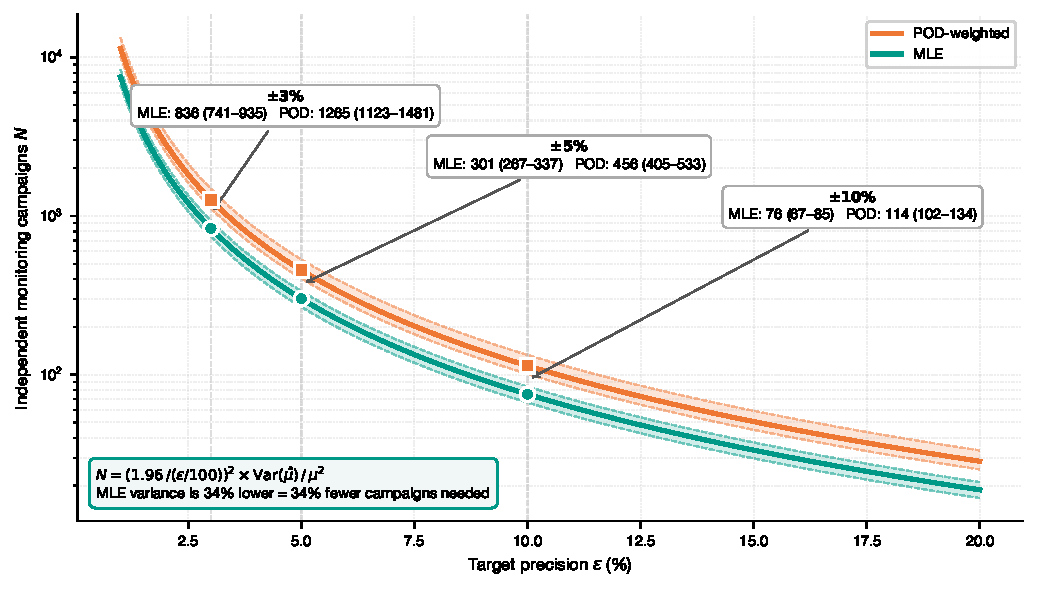
\includegraphics[width=\textwidth]{figures/figure5_precision.pdf}
\caption{Required sample size to estimate~$\mu$ within~$\pm\varepsilon\%$ at 95\% confidence, derived analytically from the single-experiment variance via equation~(\ref{eq:sample_size}). Shaded bands propagate the empirical 2.5th and 97.5th percentiles of the 25 within-batch variances. Counts are rounded upward; the normal-approximation calculation assumes independent campaigns and negligible bias. Annotated boxes give the required number of campaigns at three precision targets ($\pm 3\%$, $\pm 5\%$, $\pm 10\%$), with ranges in parentheses. Because variance scales linearly into $N$, the MLE's \edit{34\%} variance reduction translates directly into \edit{34\%} fewer required campaigns at every precision level.}
\par\smallskip
{\small\textit{Alt text:} Line chart of the number of monitoring campaigns required to estimate the mean emission rate within a given percentage precision at 95 percent confidence, for the MLE and the probability-of-detection-weighted estimator, with shaded bands from batch variance percentiles. At 3, 5 and 10 percent precision the MLE requires about 836, 301 and 76 campaigns, compared with 1,265, 456 and 114 for the probability-of-detection-weighted estimator.}
\label{fig:precision}
\end{figure}

The same variance reduction also improves the ability to detect emission changes over time. In a before--after comparison where $N$ sites are surveyed before and after an intervention, the width of the confidence interval for the change in mean emissions scales with $\sqrt{\mathrm{Var}(\hat{\mu})/N}$. Lower variance therefore means that smaller true changes become statistically distinguishable from zero. For example, a normal-approximation calculation for two independent groups with equal variances, a two-sided 5\% test, and 80\% power to detect a 20\% difference from the baseline mean gives 77 campaigns per group for MLE and 117 for POD weighting, rounding upward. For fixed group sizes, the corresponding detectable difference is about 19\% smaller with MLE. A paired before--after design additionally requires the covariance between repeated measurements; these counts do not model that covariance.

More broadly, our simulation framework provides variance as a function of the design parameters $(p_{\text{snap}}, p_{\text{cont}}, T_{\text{cont}}, \theta_{\text{snap}})$, which enables principled survey optimization that can be re-optimized as sensors improve. A monitoring program with a fixed budget can independently choose its snapshot frequency and continuous deployment rate: increasing the continuous monitoring does not mechanically reduce the snapshot survey frequency. This allocation can be framed as minimizing estimator variance subject to a budget constraint, where the cost structure depends on the specific platforms deployed (e.g., satellite tasking versus ground-based sensors). The single-parameter sweeps quantify performance along the tested designs; optimizing combinations of design parameters requires additional joint-design simulations. An optimal design will also depend on site-specific factors: relative technology costs, expected emission persistence, and available infrastructure.


\newpage

\section{Discussion}
\label{sec:discussion}

\new{Our results establish that explicit modeling of the latent emission state recovers temporal information that POD-weighted estimators discard, with material consequences for the precision of time-averaged emission estimates from heterogeneous monitoring data. This section examines the assumptions on which those results rest, the regimes in which the variance gains are most consequential, and the extensions the framework supports. We organize the discussion around three themes: the spatial scale at which the estimator operates, the sensitivity of the inference to the parametric assumptions of the model, and the practical considerations of survey cadence and noise-model realism, which will govern deployment in real monitoring programs.}

Our framework estimates emissions at the spatial scale at which individual measurements are made. For ground-based CMS and aircraft, this is typically a single facility; for satellites, it depends on instrument resolution. \edit{High-resolution instruments (e.g., those with sub-50-m pixel sizes)} can isolate individual facilities, while lower-resolution instruments may aggregate multiple sources within a single pixel.
The framework applies at whatever scale the instrument resolves: if a pixel contains multiple sources, the estimated rate represents the aggregate and the ON/OFF dynamics reflect whether any source within the pixel is active. Basin-scale estimation then proceeds by aggregating facility-level estimates, propagating uncertainty through the sum.

Several assumptions deserve discussion. The two-state Markov model assumes discrete ON/OFF switching with constant transition probabilities, whereas real emissions may vary continuously and depend on operational factors that change over time. The most consequential violations are likely to be time-of-day or seasonal effects that modulate emission frequency (e.g., tank flashing driven by temperature cycles), since these induce non-stationarity in $p_{\text{on}}$ and $p_{\text{off}}$. If these patterns are known, the analysis can be restricted to a period with approximately constant transition probabilities. Otherwise, the fitted probabilities describe average behaviour over the window, and sensitivity to non-stationarity needs to be assessed. Model misspecification can affect the estimated mean even when sampling is independent of emission activity.

We assume POD curves are known from controlled release experiments~\citep{Sherwin2021, Bell2022, ElAbbadi2024, chen2024comparing, mcmanemin2026controlled, Reuland2026}, though in practice detection probability varies with atmospheric conditions, background surface coverage, topographic conditions, and viewing geometry. Prior campaigns were mostly performed in very sunny and homogeneous surface conditions, which are optimal for air- and space-based remote sensing, and provide very simple wind patterns for CMS inference. POD misspecification would propagate into the IPW weights and the HMM emission probabilities. Systematic overestimation of POD would underweight detected events and overcount non-detections as true OFF states, biasing $\hat{\mu}$ downward; the reverse would produce upward bias. The magnitude of this effect depends on how much the true POD deviates from the assumed curve across the emission-size range that contributes most to total flux. \edit{We characterize this sensitivity quantitatively in SI, Section~\ref{SI-sec:misspec_SI}, where we perturb the assumed POD and noise parameters around their true values and report total mean squared error; these experiments assess sensitivity to calibration uncertainty under the simulated deployment.}

\edit{We use log-normal event sizes to generate the simulations, but estimate their distribution from IPW-weighted plume sizes without fitting a lognormal family. This correction requires detections across the relevant size range; reweighting cannot reliably recover events in a range that is rarely or never detected. Uncertain event assignments, noisy size estimates, interpolation of event-detection probabilities, and campaign boundaries can contribute residual bias. Retaining event sizes in the likelihood accounts for dependence between repeated detections; the event assignments and size distribution are still estimated. Joint likelihood fitting or regularized estimation of the size distribution could address some of these approximations.}


\new{The baseline scenario assumes approximately three snapshot observations per day, which approaches the upper bound of currently feasible coordinated deployments; routine single-platform operations are typically an order of magnitude sparser. Estimator variance grows as cadence decreases for any method, but the snapshot cadence sweep in Section~\ref{sec:sweeps_main} shows that the MLE's variance advantage over the POD-weighted baseline holds across cadences spanning monthly surveys to several observations per day. At the sparsest cadences, data alone are too limited for any method to recover the time-averaged rate at the single-facility level (SI, Section~\ref{SI-sec:sparse_SI}), and pooling across comparable facilities becomes necessary regardless of the estimator used.}


\new{The lognormal noise specification in equation~\eqref{eq:noise} captures the approximately scale-invariant relative error observed in controlled-release tests of aerial and satellite platforms. It does not, however, reflect the behavior of fenceline continuous monitors, whose error distributions are typically left-censored: rates below an instrument-specific floor are reported as zero rather than as small positive values. Accommodating such a distribution within the framework requires replacing equation~\eqref{eq:noise} with a censored lognormal. The downstream implications for plume identification, IPW weights, and the HMM forward algorithm merit dedicated treatment and constitute a priority for future work on fenceline applications.}

Natural extensions of this work include multi-state models (e.g., distinguishing low and high emission regimes), hierarchical models that pool information across similar facilities to improve estimates at sparsely observed sites, spatial aggregation frameworks that extend the likelihood to jointly model multiple co-located sources, and sequential updating schemes for real-time operational monitoring.


\section{Conclusion}
\label{sec:conclusion}

We have presented an iterative plug-in framework with conditional maximum-likelihood updates for estimating time-averaged methane emissions from heterogeneous monitoring data. The method jointly models emission intermittency and size-dependent detection bias, extracting information from both detections and non-detections across technologies with different sensitivities and sampling cadences.

In simulations calibrated to intensive monitoring scenarios, the method achieves 34\% variance reduction relative to POD-weighted estimation under baseline conditions, with gains varying with emission persistence and monitoring coverage. These reductions translate directly into lower sample-size requirements: for a given precision target, fewer independent monitoring campaigns are needed under the variance-based planning assumptions.

Because sensor characteristics enter as modular inputs, the framework accommodates new instruments without structural changes to the estimator. As the methane monitoring landscape continues to diversify, principled methods for combining these data streams become increasingly important. Our framework provides a statistical foundation for doing so, using temporal structure and non-detection information in modern monitoring records to support accurate, measurement-based emission estimates.

%=============================================================================
\section*{Conflicts of Interest}
%=============================================================================

The authors declare no competing interests.

%=============================================================================
\section*{Funding}
%=============================================================================

This work was partially supported by the California Energy Commission (SUMMATION project, agreement number PIR-17-015).

%=============================================================================
\section*{Data Availability}
%=============================================================================

The simulation and estimation code, parameter configurations, generated simulation datasets, and plotting scripts supporting this study are publicly available at \url{https://github.com/pburdeau/methane-mle}. The repository includes instructions for reproducing the analyses and figures.

%=============================================================================
\section*{Author Contributions}
%=============================================================================

P.B. developed the methodology, designed and ran the simulations, analyzed the results, and wrote the manuscript. E.S. and A.B. provided guidance on methodology and applications and contributed to manuscript revision.

%=============================================================================
\section*{Acknowledgments}
%=============================================================================

This work does not necessarily represent the views of the Energy Commission, its employees, or the State of California. The Energy Commission, the State of California, its employees, contractors, and subcontractors make no warranty, express or implied, and assume no legal liability for the information in this report; nor does any party represent that the uses of this information will not infringe upon privately owned rights. This paper has not been approved or disapproved by the California Energy Commission, nor has the California Energy Commission passed upon the accuracy or adequacy of the information in this paper. This manuscript has been authored by authors at Lawrence Berkeley National Laboratory under Contract No. DE-AC02-05CH11231 with the U.S. Department of Energy. The U.S. Government retains, and the publisher, by accepting the article for publication, acknowledges, that the U.S. Government retains a nonexclusive, paid-up, irrevocable, worldwide license to publish or reproduce the published form of this manuscript, or allow others to do so, for U.S. Government purposes.

The authors used Claude (Anthropic) and Codex (OpenAI) to assist with writing and debugging code throughout the project, including the simulation, estimation, and analysis code and the plotting scripts used to produce the figures, and with editing the manuscript text for clarity and concision. Numerical result figures were generated from simulation outputs. The authors retain responsibility for reviewing and validating the AI-assisted code, analyses and text, and for the content of this paper.

%=============================================================================
% Bibliography
%=============================================================================
\bibliographystyle{oup-abbrvnat}
\bibliography{references}

\end{document}
